\documentclass[12pt, doublespace, oneside]{article}
\usepackage[utf8]{inputenc}
\usepackage{multirow}
\usepackage{physics}
\usepackage{float}
\usepackage{amsfonts}
\usepackage{graphicx}
\usepackage[english]{babel}
\usepackage{hyperref}
\usepackage{nicefrac}
\let\endtitlepage\relax
\usepackage{geometry}
    %\usepackage{showframe} %This line can be used to clearly show the new margins

\newgeometry{hmargin={24mm,24mm}}   % set the margins

\renewcommand{\baselinestretch}{1.3}

\title{{\vspace{-1.5cm}}East-West Method Analysis over the All Triggers Dataset}
\author{E.Coronel\footnote{evelyn.coronel@ib.edu.ar} ,  S. Mollerach}
\date{March 2021}

\begin{document}

\begin{titlepage}
\maketitle
\end{titlepage}



% El método de Rayleigh se basa en ajustar el flujo de CRs en función de la ascensión recta $\alpha$ mediante una función armónica. El mismo permite calcular la amplitude y phase de la anisotropía para distintos armónicos, además de la probabilidad de detectar la misma señal debido a fluctuaciones de una distribución isótropa de RCs. La dificultad de utilizar el método Rayleigh recae en su sensibilidad a efectos sistemáticos: efectos del clima, variaciones en el área del Observatorio, y la sensibilidad de los instrumentos deben tenerse en cuenta.  Los efectos mencionados deben ser corregidos de la señal medida de los eventos, ya que los mismos inducen modulaciones espurias en el análisis.


There are mainly two techniques are used in the study of large-scale anisotropies over the events rate measured by the Pierre Auger Observatory: Rayleigh and East-West methods. These methods are based on studying modulations over the cosmic rays flux $I_{\alpha, \delta}$ using harmonic functions, where $\alpha$ and $\delta$ stand for the right ascension and declination respectively. 

Given an energy range, the Rayleigh analysis uses the rate of events to estimate the amplitude and phase of an anisotropy between this range up to any order. Also, using the Rayleigh distribution, it is possible to obtain the probability of measuring the same amplitude magnitude as a fluctuation of an isotropic distribution of cosmic rays. This method has approximately a resolution of $\nicefrac{1}{n}$ cycles per year where $n$ is the period of the time to be analyzed \cite{resolucion_barrido}, therefore this method might be sensible to weather modulation in the signal measured by the Observatory or area variations over the surface detectors array. To use this method properly,  instrumental effects must be kept as low as possible because these effects induce spurious amplitudes in the analysis.



% El método East - West consiste en el ajuste de una función armónica a la diferencia entre los flujos de eventos provenientes del Este y del Oeste. Si se consideran que las modulaciones espurias producidas por los efectos atmosféricos y sistemáticos son las mismas en ambas direcciones, la diferencia de flujos remueve estos efectos sin realizar correcciones adicionales. Una desventaja de este método es que su sensibilidad es menor que la del método de Rayleigh \cite{taborda}.

In the other hand, the East-West method consists of the harmonic function's approximation of the difference of rate of events measured by the Observatory arriving from the East and West directions recorded at a given sidereal time angle $\alpha^0$, i.e. the zenith's right ascension. The instrumental effects are removed for the analysis without any further corrections, but a downside of this method is its lower sensibility than the Rayleigh analysis \cite{taborda}.

% El objetivo del método  East - West es estimar la modulación dipolar de  $I(\alpha^0)$ a partir de la diferencia $I^{obs}_E -  I^{obs}_O$ mediante un análisis similar al método de  Rayleigh que se muestra en la Ec.\ref{eq:general-1-ray}, salvo modificaciones para tener en cuenta la dirección de los eventos. 
% \begin{equation}
%     I^{obs}_E -  I^{obs}_O = \frac{N}{2\pi} r_{EW} \cos(\alpha^0 -  \phi_{EW}) \label{eq:ray_ew_like}
% \end{equation}
% donde a diferencia de la expresión original, la amplitude $r_{EW}$ y phase $\phi_{EW}$ no son la amplitude y phase de la modulación en ascensión recta. Las mismas están asociadas a la modulación en la diferencia de flujos, a continuación se explica como se relacionan con $r_1$ y $\phi$  a partir del   método East - West.

Using a dipolar approximation, the East-West method estimates the modulation over the CR flux $I(\alpha^0)$ given by $I^{obs}_E -  I^{obs}_O$ in the following way:
\begin{enumerate}
    \item Given $N$ events to study, first we obtain the parameters $a_{EW}$ and $b_{EW}$:
    \begin{align}
        a_{EW} = \frac{2}{N} \sum^N_{i=1}\cos(\alpha^0_i - \beta_i) \qquad
        b_{EW} = \frac{2}{N} \sum^N_{i=1}\sin(\alpha^0_i - \beta_i)
    \end{align}
    where $\alpha^0_i$  is the Observatory's zenith right ascension at the moment of measurement of the $i$ event and $\beta_i=\pi$ if the event came from the East, $\beta=0$ otherwise.  
    \item Then we compute the amplitude and phase of the first orden approximation $r$ y $\phi$,
    \begin{tabular}{@{}p{.4\linewidth}@{}p{.5\linewidth}@{}}
        \begin{align}
            r_{EW} = \sqrt{a_{EW}^2 + b_{EW}^2} \\
            r   =\frac{\pi}{2} \frac{\langle\cos\delta \rangle}{\langle\sin\theta \rangle} r_{EW}\label{dperp} 
        \end{align}
        &    \begin{align}
            \phi_{EW} = \arctangent{\frac{b_{EW}}{a_{EW}}} \\
            \phi = \phi_{EW}+ \frac{\pi}{2} \label{phase_fisico}
        \end{align}
      \end{tabular}
      where the amplitude $r_{EW}$ and phase $\phi_{EW}$ are related to  $r$ y $\phi$, which are the amplitude and phase of the modulation of the first order's approximation. The values $\langle\cos\delta \rangle$ and $\langle\sin\theta \rangle$ are the mean value over all the events $i$.

      \item To generalize this analysis to any frequency, instead of using the variable $\alpha^0$ we used the variable:
      $\tilde{\alpha} = 2\pi f_x t_i $, where $f_x$ stands for the  frequency  of interest, and $t_i$ is the time in which the event was measured. It allows us to study the amplitude over solar frecuency to verify the weather modulation over the SD signal.

      \item Another variable used in this article is the component of the dipole amplitude $d_\perp$ in the equatorial plane. It can be calculated using the following expression:
      \begin{equation}
        d_{\perp} = \frac{\pi}{2\langle\sin\theta \rangle} r_{EW} \label{dperp} 
      \end{equation}
      
\end{enumerate}
% Finally we have all the parameters needed to estima

% \begin{equation}
%     I^{obs}_E -  I^{obs}_O = \frac{N}{2\pi} r_{EW} \cos(\alpha^0 -  \phi_{EW}) \label{eq:ray_ew_like}
% \end{equation}
% where the amplitude $r_{EW}$ and phase $\phi_{EW}$ are related to  $r$ y $\phi$, which are the amplitude and phase of the modulation of the first order's approximation.

% \begin{tabular}{@{}p{.4\linewidth}@{}p{.5\linewidth}@{}}
%     \begin{align}
%         d_{\perp} = \frac{\pi}{2\langle\sin\theta \rangle} r_{EW} \label{dperp} \\
%         r_1   =\frac{\pi}{2} \frac{\langle\cos\delta \rangle}{\langle\sin\theta \rangle} r_{EW} \label{r_fisico}  \\
%         \alpha_d = \phi_{EW} + \frac{\pi}{2} \label{phase_fisico}
%     \end{align}
%     &    \begin{align}
%         \sigma_{x,y} = \frac{\pi}{2\langle\sin\theta \rangle} \sqrt{\frac{2}{N}}\\
%         \sigma   = \frac{\pi \langle\cos\delta \rangle}{2\langle\sin\theta \rangle} \sqrt{\frac{2}{N}}
%     \end{align}
%   \end{tabular}

% En este capítulo se presentan los resultados obtenidos mediante el método East-West con los eventos de All Triggers, para  distintos rangos de energía. Estos resultados se comparan con los valores obtenidos en \cite{Aab_2020} sobre los eventos  del Disparo Estándar. 

In this article, we present the novel results over the All Triggers dataset. The results were calculated using the East-West method for different energy ranges and were compared with other published results obtained with the Herald dataset by the Collaboration.

\section{Datasets characteristics}

% Los eventos son clasificados en los distintos rangos mediante la energía reportada por la Colaboración. El conjunto de eventos registrados con All Triggers abarca los años 2014 y 2019, y para el Disparo Estándar se listan eventos medidos entre el 2004 y 2018. Las características de estos dos conjuntos de datos se especifican en la Tabla 
\paragraph{} The following events are classified by their energy, as they were reported by the Collaboration. These events are used to report and compare several results. The All Triggers dataset includes registered events from 2014 to 2020. Meanwhile, the Herald dataset contains data gathered from 2004 to 2018. The characteristics of both datasets are presented in Table \ref{tab:datasets}

\begin{table}[H]
    \begin{small}
        \begin{center}
            \begin{tabular}{lc|l|l|l|}
\hline
\multicolumn{1}{|l|}{\multirow{4}{*}{\begin{tabular}[c]{@{}c@{}}Time\\ span\end{tabular}}}    & All Triggers        & From  &\multicolumn{2}{l|}{January 1$^{st}$, 2014 } \\ \cline{3-5} 
\multicolumn{1}{|l|}{}                                                                            & 6 years             & To    &\multicolumn{2}{l|}{January 1$^{st}$, 2020} \\ \cline{2-5} 
\multicolumn{1}{|l|}{}                                                                            & Herald              & From  &\multicolumn{2}{l|}{January 1$^{st}$, 2004} \\ \cline{3-5}
\multicolumn{1}{|l|}{}                                                                            & 14.7 years          & To    &\multicolumn{2}{l|}{August 1$^{st}$, 2018} \\ \hline  \\

\hline                                                                          \multicolumn{2}{|c|}{Energy range [EeV]}                                                    & \multicolumn{1}{c|}{0.25 - 0.5}  & \multicolumn{1}{c|}{ 0.5  - 1 } &\multicolumn{1}{c|}{ 1 - 2 } \\ \hline
\multicolumn{1}{|l|}{\multirow{2}{*}{Events}}                            & All Triggers    & $3\,967\,368$     & $3\,638\,226$   & $1\,081\,846$ \\ \cline{2-5} 
\multicolumn{1}{|l|}{}                                                    & Herald & $770\,316$        & $2\,388\,467$   & $1\,243\,103$ \\ \hline
\multicolumn{1}{|l|}{\multirow{2}{*}{\begin{tabular}[c]{@{}c@{}}Mean \\ Energy\end{tabular}}} & All Triggers   & $0.38$           & $0.69$         & $1.32$       \\ \cline{2-5} 
\multicolumn{1}{|l|}{}                                                                             & Herald & $0.43$            & $0.70$          & $1.28$       \\ \hline
\end{tabular}
            \caption{Datasets characteristics for several energy ranges.}
            \label{tab:datasets}
        \end{center}
    \end{small}
\end{table}



\section{Results of the East-West Analysis}
\subsection{Results in the 0.25 EeV - 0.5 EeV energy range}

En la Tabla \ref{tab:primer_bin_data} se presentan los resultados para este rango de energía en las frecuencias solar y sidérea de All Triggers. Los mismos  se comparan con resultados con el Disparo Estándar que fueron reportados en \cite{Aab_2020}. Los valores de $\sigma$ de All Triggers es la mitad que el valor reportado para el Disparo Estándar,  esto se debe a que el primer conjunto de datos tiene registrados $\sim 5$  veces más eventos que el segundo.

\begin{table}[H]
    \begin{small}
        \begin{center}
            \begin{tabular}[c]{l|c|c||c|}
\cline{2-4}                                       & \multicolumn{2}{c||}{All Triggers}    & \multicolumn{1}{c|}{Disparo Estándar}   \\ \hline
\multicolumn{1}{|l|}{Frequency:                } & Solar	                & Sidérea	                & Sidérea \cite{Aab_2020}   \\ \hline
\multicolumn{1}{|l|}{Amplitude r [\%]:           } & $0.17^{+0.22}_{-0.07}$	& $0.12^{+0.24}_{-0.03}$ 	& $0.5^{+0.4}_{-0.2}$ \cite{codigo}      \\
\multicolumn{1}{|l|}{$r_{99}$ [\%]:             } & \multicolumn{2}{c||}{0.58}                          & 1.1\cite{codigo}                 \\
\multicolumn{1}{|l|}{$r^{UL}$ [\%]:             } & 0.67 	                & 0.64                      & 1.4\cite{codigo}                 \\ 
\multicolumn{1}{|l|}{$\sigma$[\%]:              } & \multicolumn{2}{c||}{0.19}                          & 0.38\cite{codigo}       \\\hline
\multicolumn{1}{|l|}{Amplitude $d_\perp$[\%]:    } & -	                    & $0.16^{+0.31}_{-0.04}$ 	& $0.6^{+0.5}_{-0.3}$       \\
\multicolumn{1}{|l|}{$d_{99}$ [\%]:             } & - 	                    & 0.73                      & 1.5  \cite{codigo}                \\
\multicolumn{1}{|l|}{$d_{\perp}^{UL}[\%]$       } & -                       & 0.80                      & 1.8                         \\
\multicolumn{1}{|l|}{$\sigma_{x,y}$[\%]:        } & -	                    & 0.24	                    & 0.48       \\\hline
\multicolumn{1}{|l|}{Probabilidad      :        } & 0.66                    & 0.81	                    & 0.45       \\
\multicolumn{1}{|l|}{Phase[$^o$]:                } & 221$\pm$77              & 280$\pm$90                & 225$\pm$64\\ \hline
\multicolumn{1}{|l|}{$\langle\cos\delta \rangle$} & \multicolumn{2}{c||}{0.79}        	                & 0.79 \cite{codigo}        \\        
\multicolumn{1}{|l|}{$\langle\sin\theta \rangle$} & \multicolumn{2}{c||}{0.46}        	                & 0.52 \cite{codigo}        \\ \hline       
            \end{tabular}
            
        \end{center}
    \end{small}
    \caption{Características para las frecuencias solar y sidérea con el método East-West en el primer armónico en rango de energía 0.25 EeV - 0.5 EeV.}
    \label{tab:primer_bin_data}
\end{table}

\begin{figure}[H]
    \begin{small}
        \begin{center}
            \vspace*{-1. cm}
            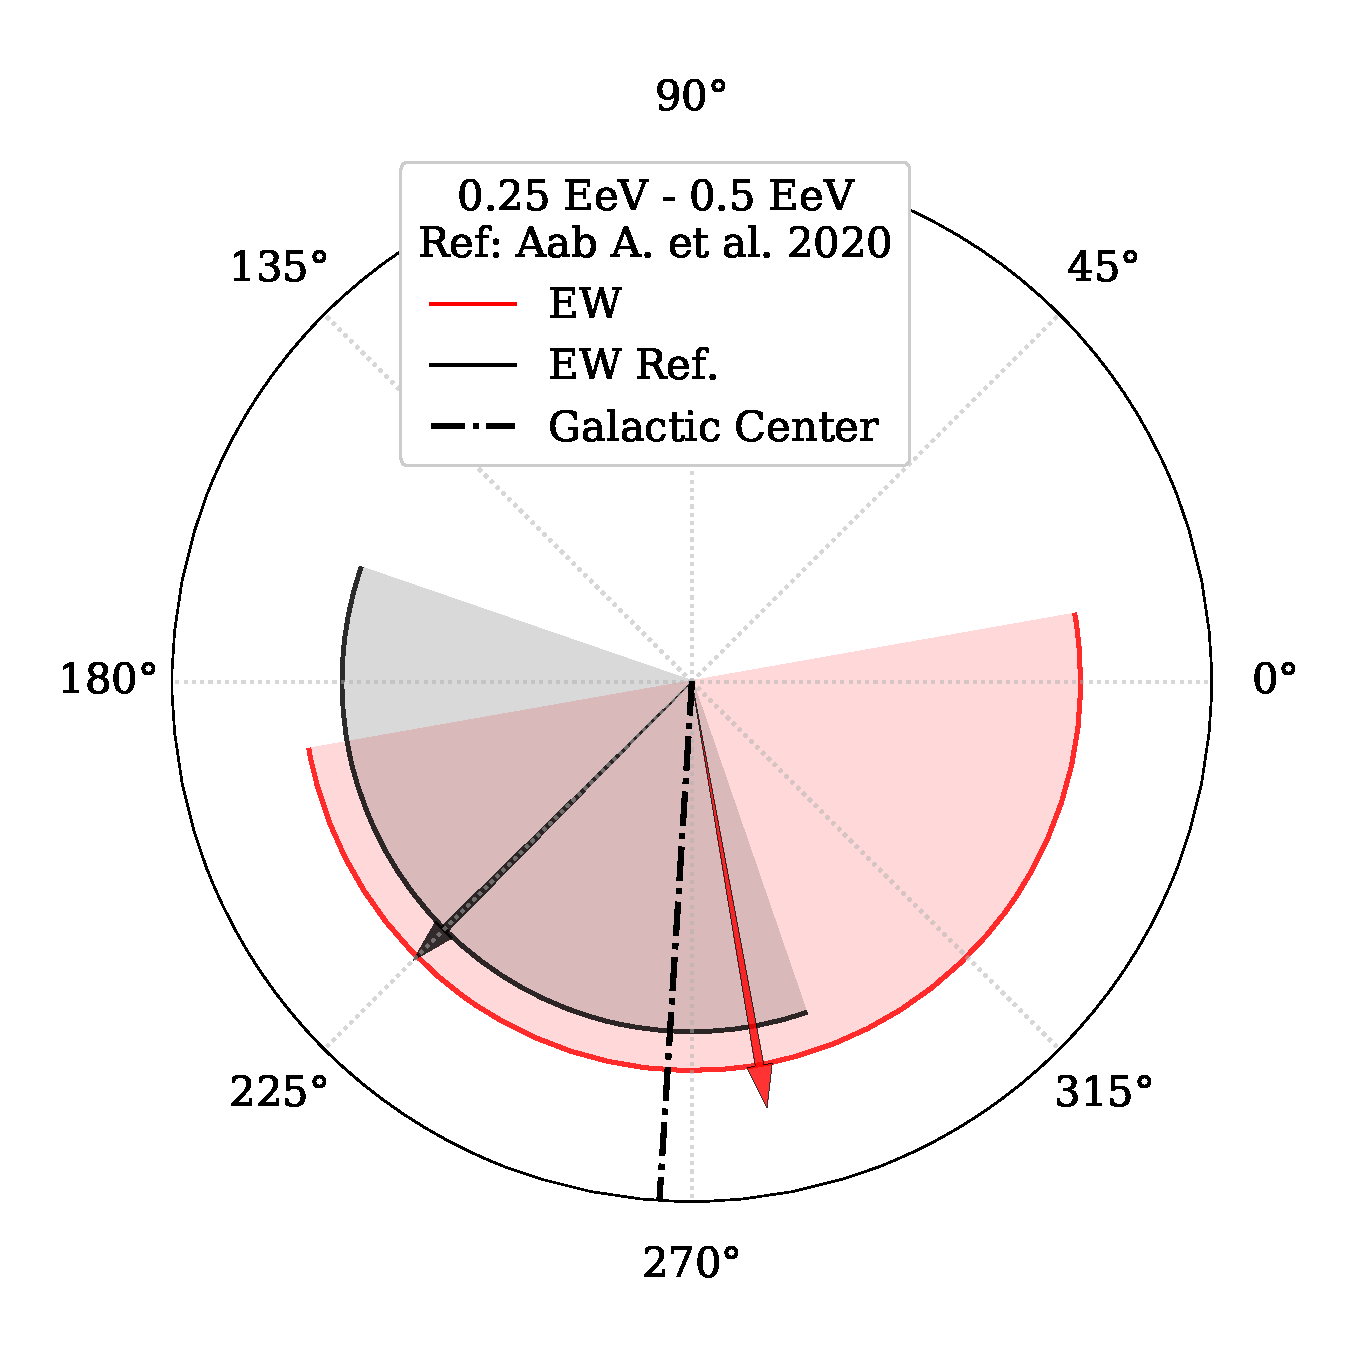
\includegraphics[width=0.65\textwidth]{Figs/phase_primer_bin_v3.pdf}
            \vspace*{-1 cm}
        \end{center}
        \caption{Valores de las fases obtenidos en este trabajo y en el trabajo Aab A. et al. (2020) \cite{Aab_2020} con sus respectivas incertidumbres para la frequency sidérea en el  rango 0.25 EeV - 0.5 EeV.}
        \label{fig:primer}
    \end{small}
\end{figure}

En la Fig. \ref{fig:primer} se comparan las  fases en frequency sidérea obtenida en este trabajo y la reportada en \cite{Aab_2020}, donde la línea punteada marca la dirección del centro galáctico.  En esta figura en la tabla anterior, se observa que la incertidumbre obtenida para la phase de All Triggers es amplia, esto se debe a que la amplitude $r$ es pequeña comparada con el valor de $\sigma$. 


Realizando el barrido de frecuencias con la variable de la Ec.\ref{ra_arb}, se obtiene que en este rango de energía las amplitudes se  distribuyen en frequency como se muestra en la Fig.\ref{fig:primer_barrido}. La línea horizontal indica el valor de $r_{99}$ para cada frequency, además se observa que ninguna amplitude supera dicho umbral.



\begin{figure}[H]
    \begin{small}
        \begin{center}
            \vspace*{-0.6 cm}
            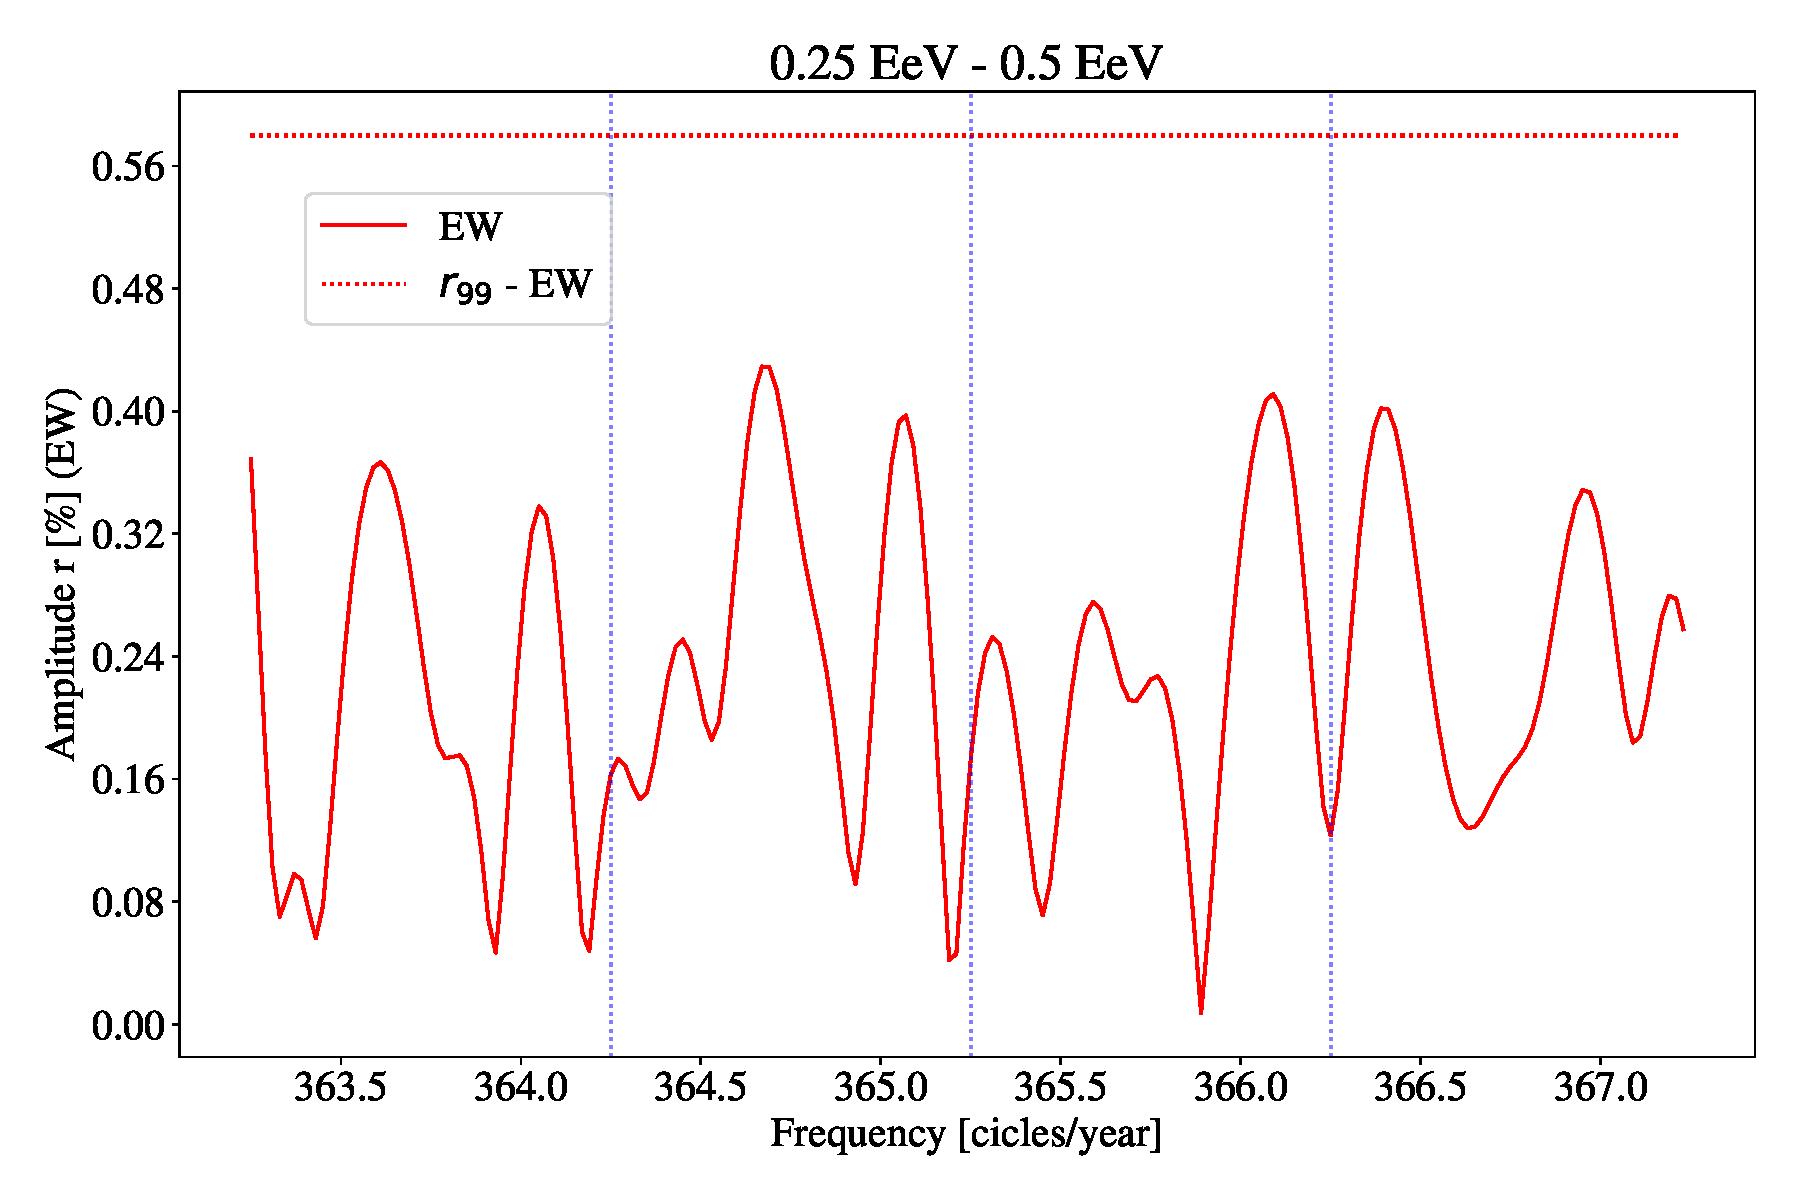
\includegraphics[width=0.9\textwidth]{Figs/plot_bin_1_barrido_v3_EW.pdf}
            \vspace*{-0.8 cm}
        \end{center}
        \caption{Barrido de frecuencias en el  rango 0.25 EeV - 0.50 EeV mediante el método East-West.}
        \label{fig:primer_barrido}
    \end{small}
\end{figure}

\subsection{Results in the 0.5 EeV - 1 EeV energy range}

En la Tabla \ref{tab:primer_bin_data} se presentan los resultados para el rango 0.5 EeV - 1 EeV en las frecuencias solar y sidérea de All Triggers, además se comparan con los resultados reportados en \cite{Aab_2020}.


El barrido de frecuencias con la variable de la Ec.\ref{ra_arb} para este rango de energía se observa en la Fig.\ref{fig:segundo_barrido}. La línea horizontal indica el valor de $r_{99}$ para cada frequency, además se observa que ninguna frequency supera dicho umbral. 


En la Fig. \ref{fig:segundo} se comparan las direcciones en las que apuntan la phase en frequency sidérea obtenida en este trabajo con la obtenida en \cite{Aab_2020}. En esta figura se observa que resultados similares entre sí en valor e incertidumbre, y apuntan a una dirección cercana al centro galáctico.



\begin{table}[H]
        \begin{small}
            \begin{center}
                \begin{tabular}[c]{l|c|c||c|}
\cline{2-4}                                       & \multicolumn{2}{c||}{All Triggers}    & \multicolumn{1}{c|}{Disparo Estándar}   \\ \hline
\multicolumn{1}{|l|}{Frequency:                } & Solar	                & Sidérea	                 & Sidérea \cite{Aab_2020}   \\ \hline
\multicolumn{1}{|l|}{Amplitude r [\%]:           } & $0.43^{+0.21}_{-0.14}$	& $0.44^{+0.21}_{-0.14}$ 	& $0.38^{+0.20}_{-0.14}$ \cite{codigo}      \\
\multicolumn{1}{|l|}{$r_{99}$ [\%]:             } & \multicolumn{2}{c||}{0.56}                          & 0.64\cite{codigo}                 \\
\multicolumn{1}{|l|}{$r^{UL}$ [\%]:             } & 0.89 	                & 0.90                      & 0.90 \cite{codigo}                 \\ 
\multicolumn{1}{|l|}{$\sigma$[\%]:              } & \multicolumn{2}{c||}{0.18}                          & 0.21 \cite{codigo}      \\\hline
\multicolumn{1}{|l|}{Amplitude $d_\perp$[\%]:    } & -	                    & $0.56^{+0.27}_{-0.18}$ 	& $0.5^{+0.3}_{-0.2}$       \\
\multicolumn{1}{|l|}{$d_{99}$ [\%]:             } & - 	                    & 0.71                      & 0.8   \cite{codigo}                \\
\multicolumn{1}{|l|}{$d_{\perp}^{UL}[\%]$       } & -                       & 1.1                       & 1.1                         \\
\multicolumn{1}{|l|}{$\sigma_{x,y}$[\%]:        } & -	                    & 0.23	                    & 0.21       \\\hline
\multicolumn{1}{|l|}{Probabilidad      :        } & 0.065                   & 0.055	                    & 0.20       \\
\multicolumn{1}{|l|}{Phase[$^o$]:                } & 205$\pm$34              & 258$\pm$34                & 261$\pm$43\\ \hline
\multicolumn{1}{|l|}{$\langle\cos\delta \rangle$} & \multicolumn{2}{c||}{0.79}        	                & 0.79 \cite{codigo}        \\        
\multicolumn{1}{|l|}{$\langle\sin\theta \rangle$} & \multicolumn{2}{c||}{0.50}        	                & 0.54\cite{codigo}        \\ \hline       
                \end{tabular}
            \end{center}
        \end{small}
        \caption{Características para las frecuencias solar y sidérea con el método East-West en el primer armónico en rango de energía 0.5 EeV - 1 EeV}
        \label{tab:segundo_bin_data}
    \end{table}


    


    \begin{figure}[H]
        \begin{small}
            \begin{center}
                \vspace*{-1.6 cm}
                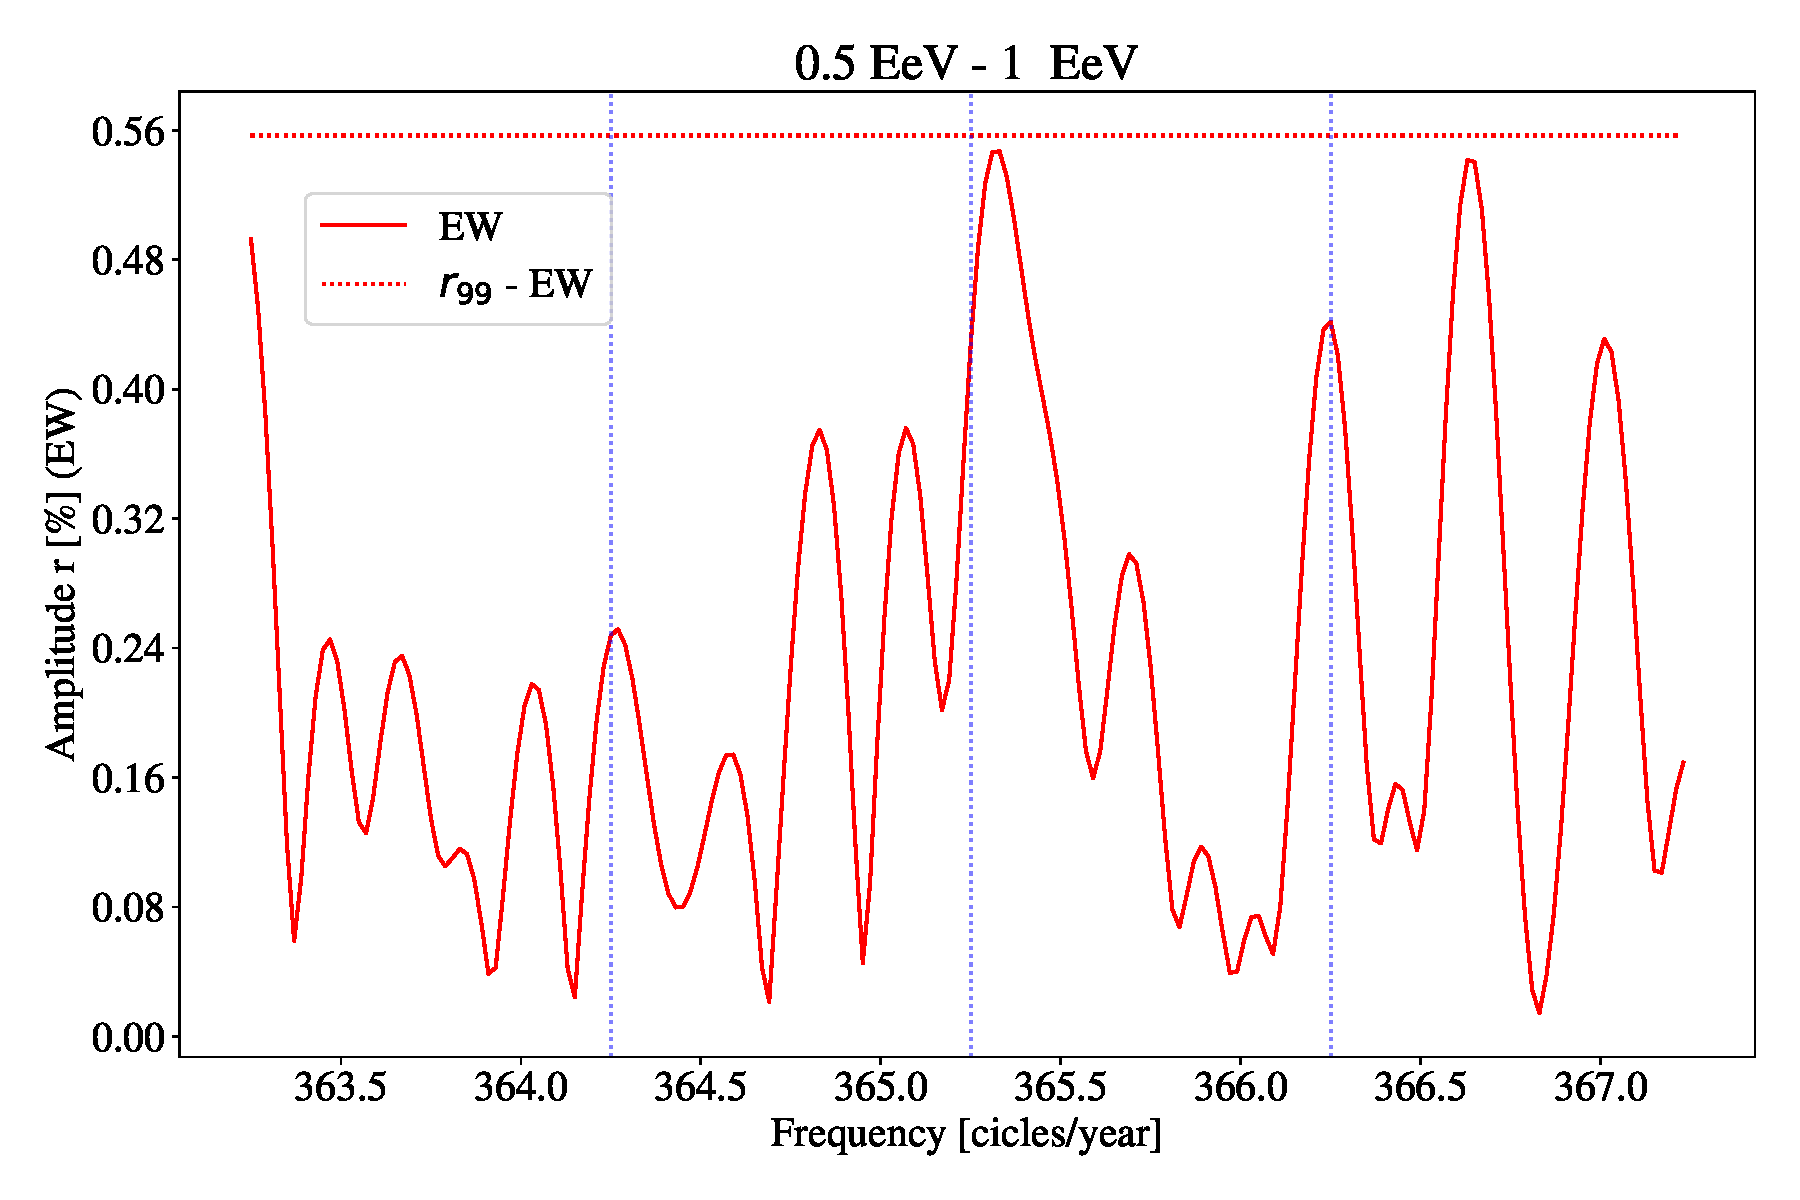
\includegraphics[width=0.9\textwidth]{Figs/plot_bin_2_barrido_v3_EW.pdf}
                \vspace*{-0.6 cm}
            \end{center}
            \caption{Barrido de frecuencias en el  rango 0.5 EeV - 1.0 EeV mediante el método East-West.}
            \label{fig:segundo_barrido}
        \end{small}
    \end{figure}    

\subsection{Results in the 1.0 EeV - 2.0 EeV energy range}
 
En las Tablas \ref{tab:solar_3}  se comparan los resultados de este trabajo  para la frequency solar. Las amplitudes están por debajo de $r_{99}$ y son compatibles entre sí.


    \begin{figure}[H]
        \begin{small}
            \begin{center}
                \vspace*{-0.65 cm}
                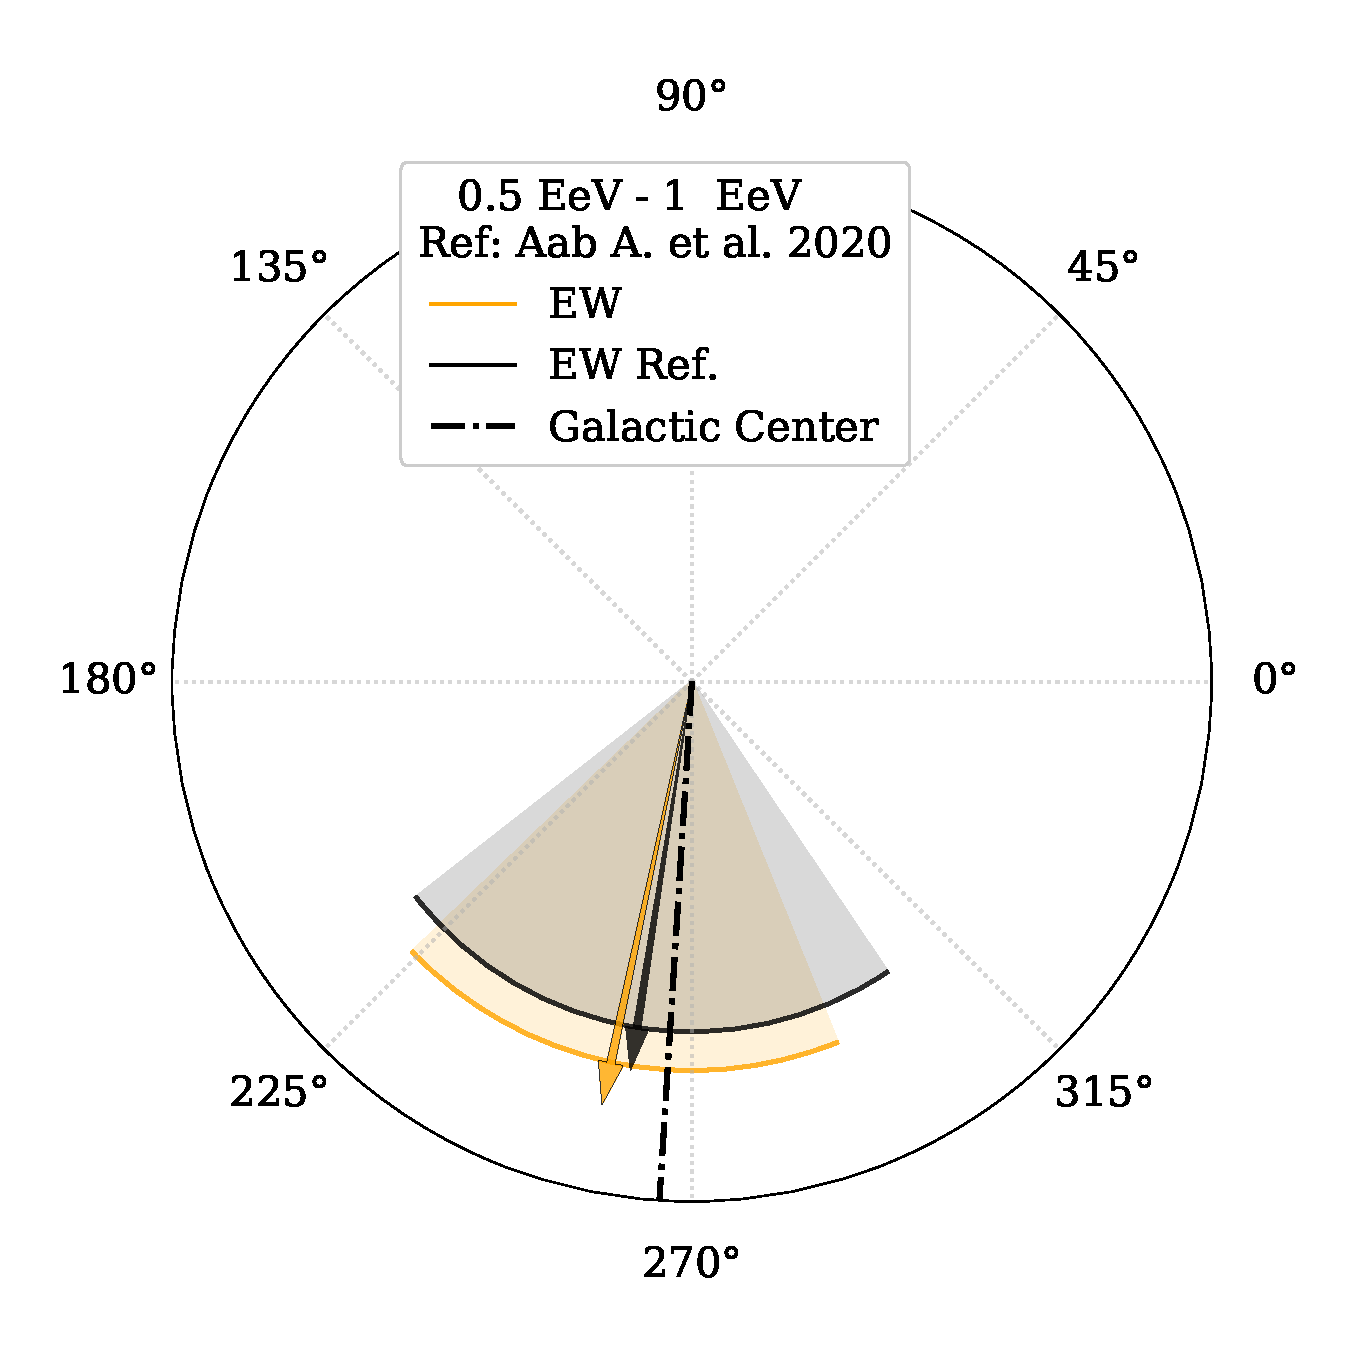
\includegraphics[width=0.65\textwidth]{Figs/phase_segundo_bin_v3.pdf}
                \vspace*{-1.1 cm}
            \end{center}
            \caption{Valores de las fases obtenidos en este trabajo y en el trabajo Aab A.  et al. (2020) \cite{Aab_2020} con sus respectivas incertidumbres para la frequency sidérea en el rango 0.5 EeV - 1.0 EeV .}
            \label{fig:segundo}
        \end{small}
    \end{figure}


    \begin{table}[H]
        \vspace*{-0.81 cm}
        \begin{small}
            \begin{center}
                \begin{tabular}[c]{l|c|c|c|}
                    \cline{2-4}         & \multicolumn{3}{c|}{All Triggers} \\ \cline{2-4}
                                        & Rayleigh   &                   & East - West            \\\hline
\multicolumn{1}{|l|}{Frequency:}       & \multicolumn{3}{c|}{Solar}        \\
\multicolumn{1}{|l|}{Amplitude $r$[\%]:} & $0.24^{+0.16}_{-0.09}$&         & $0.28^{+0.35}_{-0.11}$ \\
\multicolumn{1}{|l|}{$r_{99}$ [\%]:   } & 0.41                  &         & 0.91       \\
\multicolumn{1}{|l|}{$r_{UL}$ [\%]:   } & 0.58                  &        & 1.1       \\
\multicolumn{1}{|l|}{$\sigma$:        } & 0.14                  &         & 0.30          \\\hline
\multicolumn{1}{|l|}{Probabilidad:    } & 0.22                  &          & 0.65          \\
\multicolumn{1}{|l|}{Phase:            } & 260$\pm$48            &         & 279$\pm$76    \\\hline
                \end{tabular}
            \end{center}
            \vspace*{-0.41 cm}
        \end{small}
        \caption{Características para la frequency solar con los métodos de Rayleigh  e East-West en el primer armónico en el rango 1 EeV - 2 EeV.}
        \label{tab:solar_3}
    \end{table}
    


    En la Tabla \ref{tab:siderea_3} se comparan los resultados de este trabajo y los obtenidos en el trabajo \cite{Aab_2020} para la frequency sidérea. Para All Triggers se comparan los métodos de Rayleigh y East-West, en el primer método se obtiene que la probabilidad que la amplitude obtenida se deba al ruido es de $6.3\%$ mientras que en segundo método $26\%$. Esta diferencia entre probabilidades no puede deberse a la cantidad de eventos, porque es el mismo conjunto de datos. En la Fig.\ref{fig:tercer} se observan en una figura en coordenadas polares mostrando las fases del trabajo \cite{Aab_2020} y este trabajo para la frequency sidérea.


    El barrido de frecuencias con la variable de la Ec.\ref{ra_arb} para este rango de energía se observa en la Fig.\ref{fig:tercer_barrido}. La línea horizontal indica el valor de $r_{99}$ para cada frequency y se observa que ninguna frequency supera dicho umbral. En la frequency solar no se observa ningún pico, esto se debe a que el método East - West es robusto con respecto a las modulación del clima. Se observa un pico en sidérea pero el mismo no es significativo con respecto al $r_{99}$.


    \begin{figure}[H]
        \begin{small}
            \begin{center}
                \vspace*{-0.65 cm}
                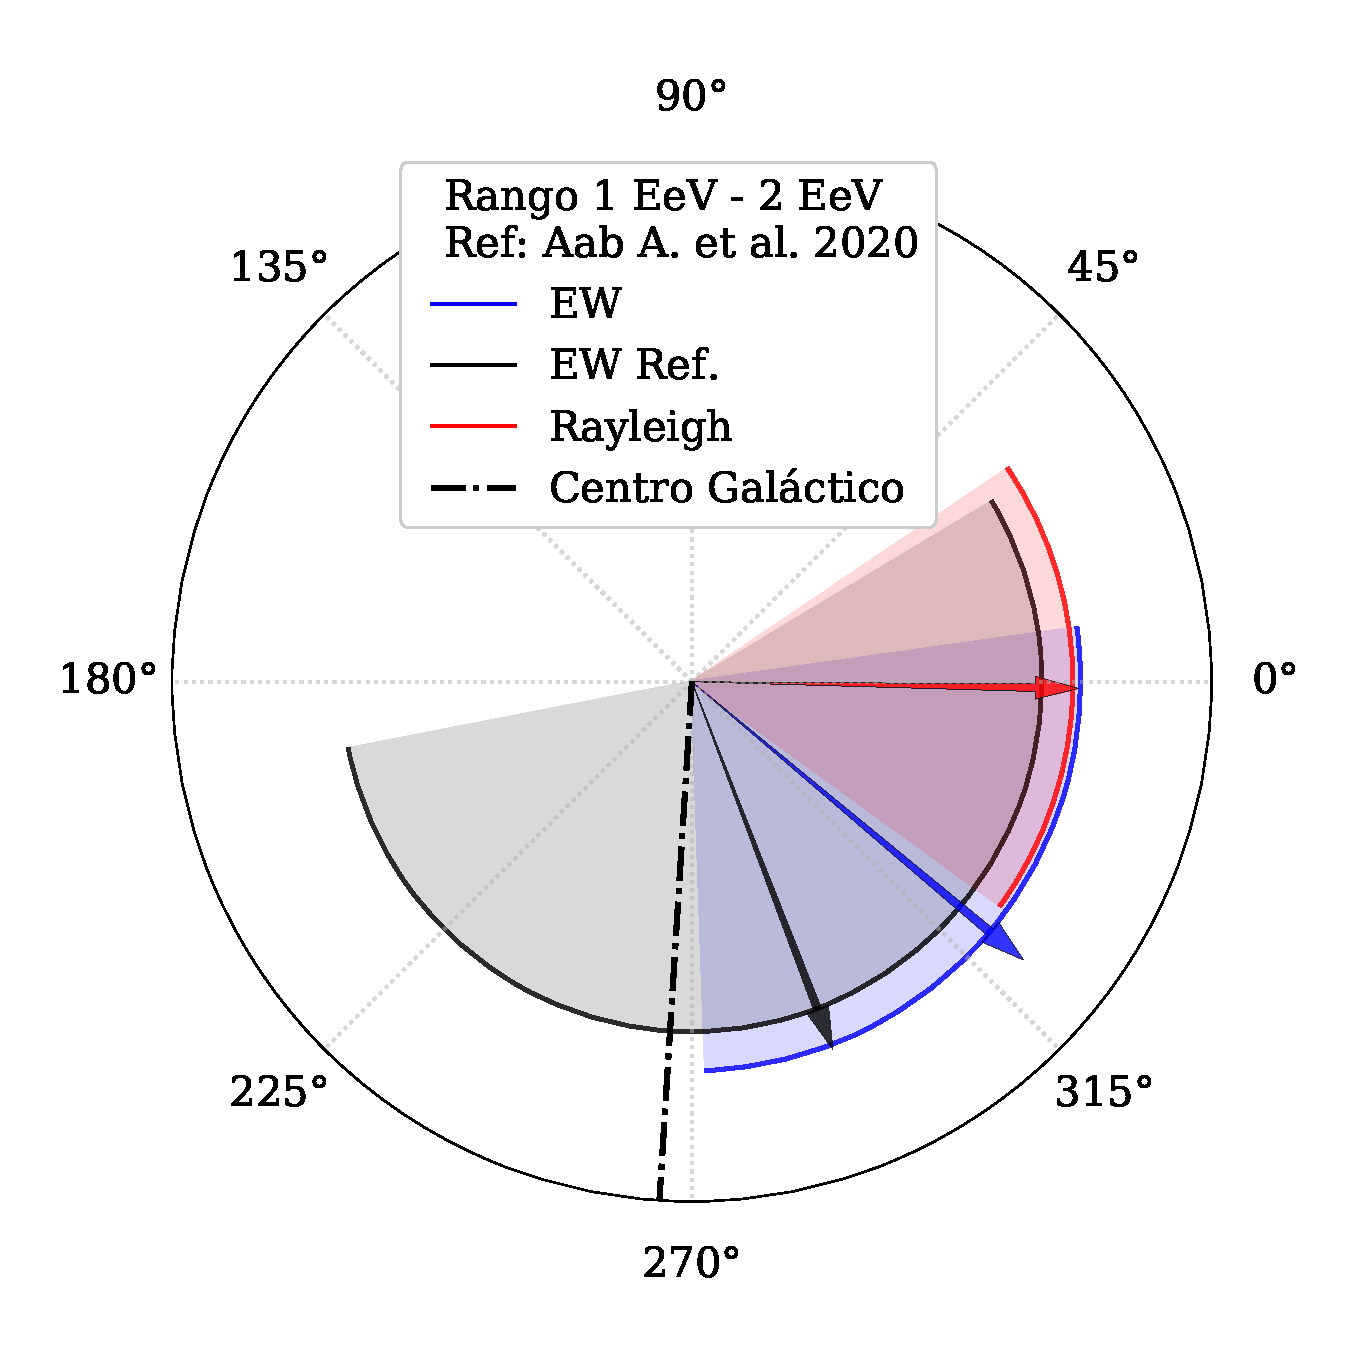
\includegraphics[width=0.65\textwidth]{Figs/phase_tercer_bin_v3.pdf}
                \vspace*{-1.2 cm}
            \end{center}
        \caption{Valores de las fases obtenidos en este trabajo y en el trabajo Aab A. et al. (2020) \cite{Aab_2020} con sus respectivas incertidumbres para la frequency sidérea en el  rango 1.0 EeV - 2.0 EeV .}
        \label{fig:tercer}
        \end{small}
    \end{figure}
    \begin{table}[H]
        \vspace*{-0.51 cm}
        \begin{small}
            \begin{center}
                \begin{tabular}[c]{l|c|c|c||c|}
                    \cline{2-5}                 & \multicolumn{3}{c||}{All Triggers}                  & Disparo Estándar      \\
                    \cline{2-5}                 & Rayleigh               &       & East - West                 & East - West\cite{Aab_2020}      \\\hline
\multicolumn{1}{|l|}{Frequency:             }  & \multicolumn{3}{c||}{Sidérea}                               & Sidérea        \\ \hline
\multicolumn{1}{|l|}{Amplitude $r$ [\%]:      }  & $0.32^{+0.16}_{-0.10}$ &  	    & $0.5^{+0.3}_{-0.2}$         & $0.14^{+0.37}_{-0.02}$\cite{codigo}       \\
\multicolumn{1}{|l|}{$r_{99}$[\%]:           }  & 0.41	                 &         & 0.91                        & 0.84\cite{codigo}        \\
\multicolumn{1}{|l|}{$r^{UL}[\%]$      }        & 0.66                   &         & 1.3                         & 0.89 \cite{codigo}        \\
\multicolumn{1}{|l|}{$\sigma$[\%]:     }        & 0.14                   &         & 0.30	                    & 0.28 \cite{codigo}          \\ \hline
\multicolumn{1}{|l|}{Amplitude $d_\perp$ [\%]:}  & $0.41^{+0.20}_{-0.13}$ &         & $0.6^{+0.4}_{-0.3}$         & $0.18^{+0.47}_{-0.02}$       \\ 
\multicolumn{1}{|l|}{$d_{99}$[\%]:           }  & 0.53	                 &        & 1.1                         & 1.1\cite{codigo}        \\
\multicolumn{1}{|l|}{$d_{\perp}^{UL}[\%]$    }  & 0.84                   &         & 1.6                         & 1.1        \\
\multicolumn{1}{|l|}{$\sigma_{x,y}$[\%]:     }  & 0.17                   &         & 0.38	                    & 0.35          \\ \hline
\multicolumn{1}{|l|}{Probabilidad:           }  & 0.063	                 &            & 0.26                        & 0.87          \\
\multicolumn{1}{|l|}{Phase[$^o$]:             }  & 357$\pm$35             &        & 320$\pm$48                 & 291$\pm$100      \\\hline
\multicolumn{1}{|l|}{$\langle\cos\delta\rangle$}&{0.78}&  &{0.78}                        & 0.78       \\        
\multicolumn{1}{|l|}{$\langle\sin\theta\rangle$}&{0.55}&  &{0.55}                        & 0.57       \\ \hline       
\end{tabular}
            \end{center}
        \end{small}
        \vspace*{-0.21 cm}
        \caption{Características para la frequency sidérea con los métodos de Rayleigh  e East-West en el primer armónico en el rango 1 EeV - 2 EeV.}
        \label{tab:siderea_3}
    \end{table}



    \begin{figure}[H]
        \begin{small}
            \begin{center}
                \vspace*{-0.21 cm}
                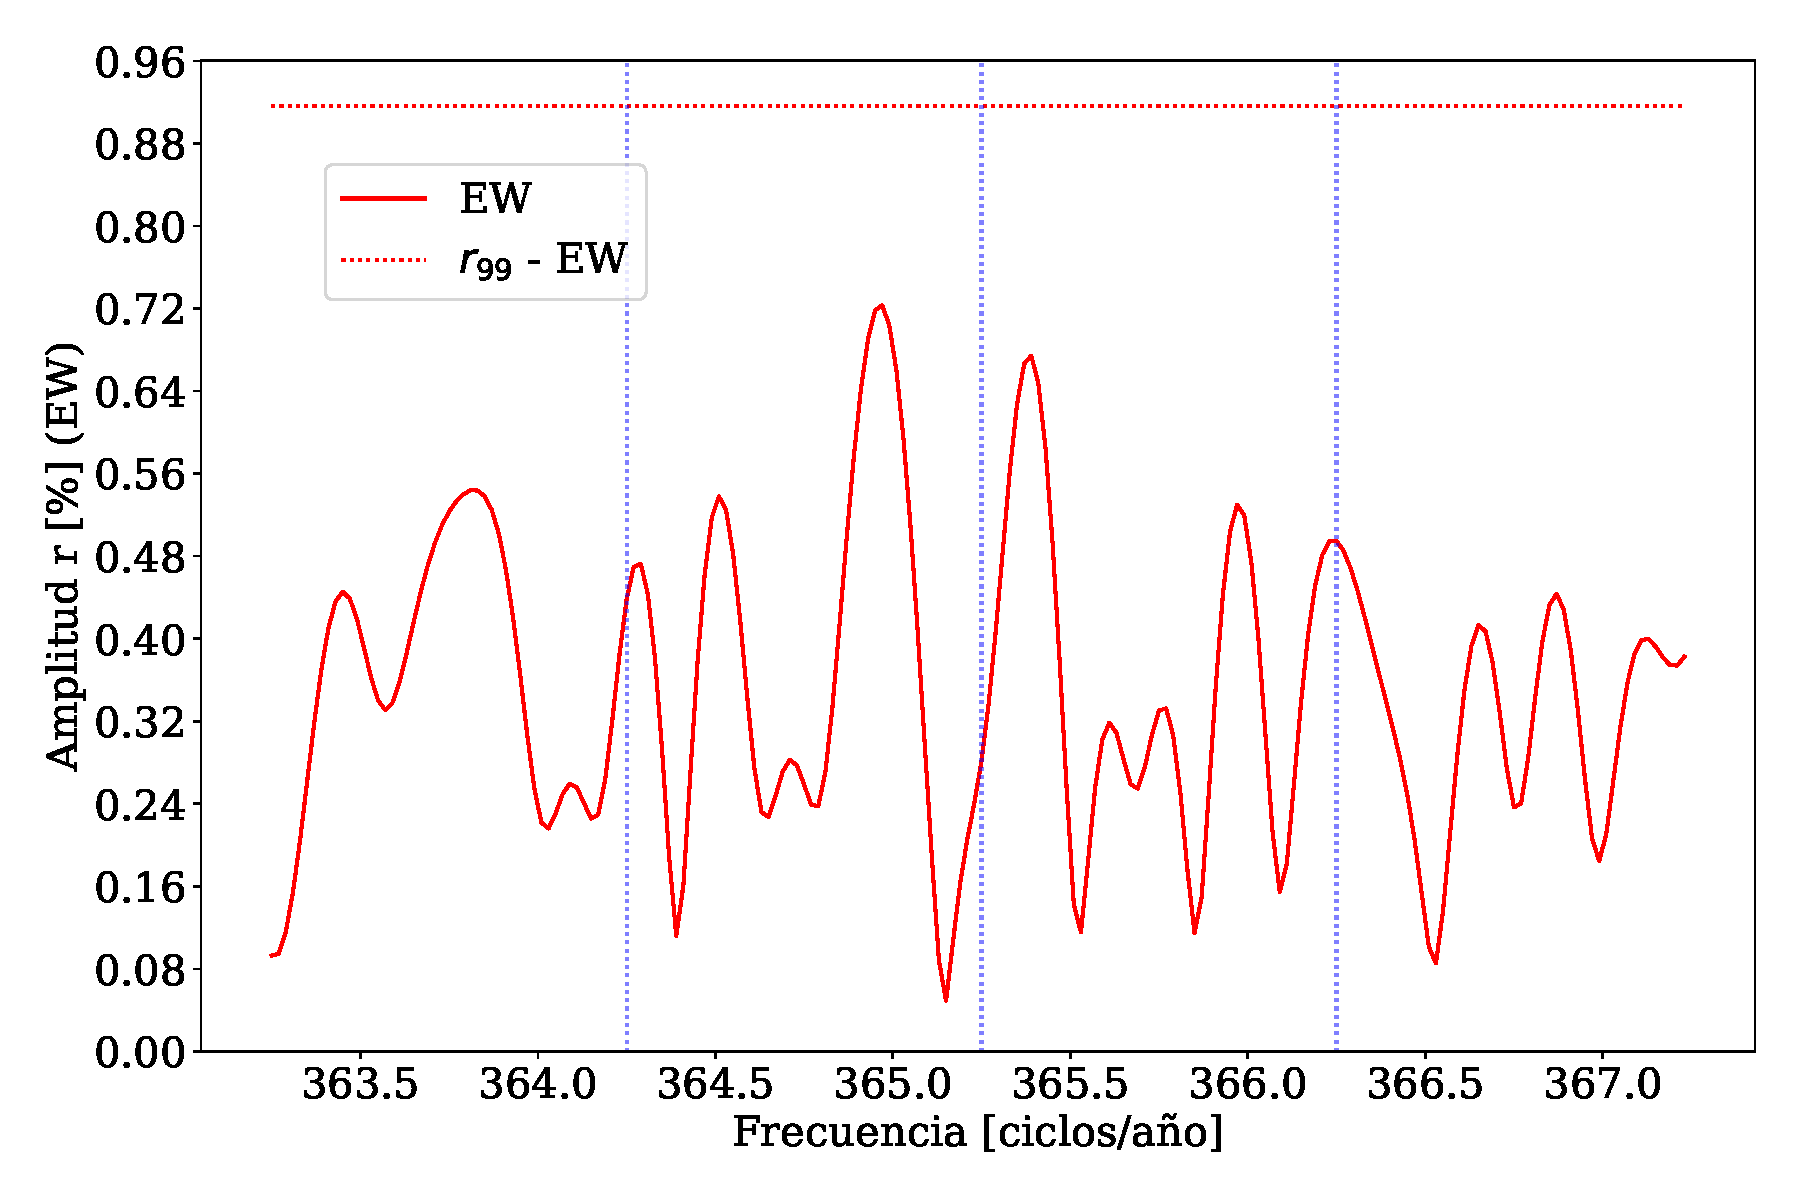
\includegraphics[width=0.9\textwidth]{Figs/plot_bin_3_barrido_v3_EW.pdf}
                \vspace*{-1 cm}
            \end{center}
            \caption{Barrido de frecuencias en el rango 1 EeV - 2 EeV mediante el método East-West.}
            \label{fig:tercer_barrido}
        \end{small}
    \end{figure}    


    \section{Análisis de los resultados}

    El barrido de frecuencias para el conjunto de datos de All Triggers contiene datos de 6 años. Este rango de tiempo  permite tener una resolución de $\sim\nicefrac{1}{6}  \,$ciclos/año \cite{resolucion_barrido}. Los picos obtenidos en los barridos presentados en las Figs.\ref{fig:primer_barrido}, \ref{fig:segundo_barrido} y \ref{fig:tercer_barrido} están distanciados en promedio $\nicefrac{1}{5}\,$ciclos/año entre sí por lo que están dentro de la resolución posible del análisis. 

    % Para poder comparar los resultados de $d_\perp$ entre sí, podríamos graficar los valores de la proyección y de la límite del $99\%$ como se muestra en la Fig.\ref{fig:no_normalizado}. El inconveniente es la cantidad de datos en cada rango de energía entre los conjuntos de datos, All Triggers y Disparo Estándar, son distintos.

    % \begin{figure}[H]
    %     \begin{small}
    %         \begin{center}
    %             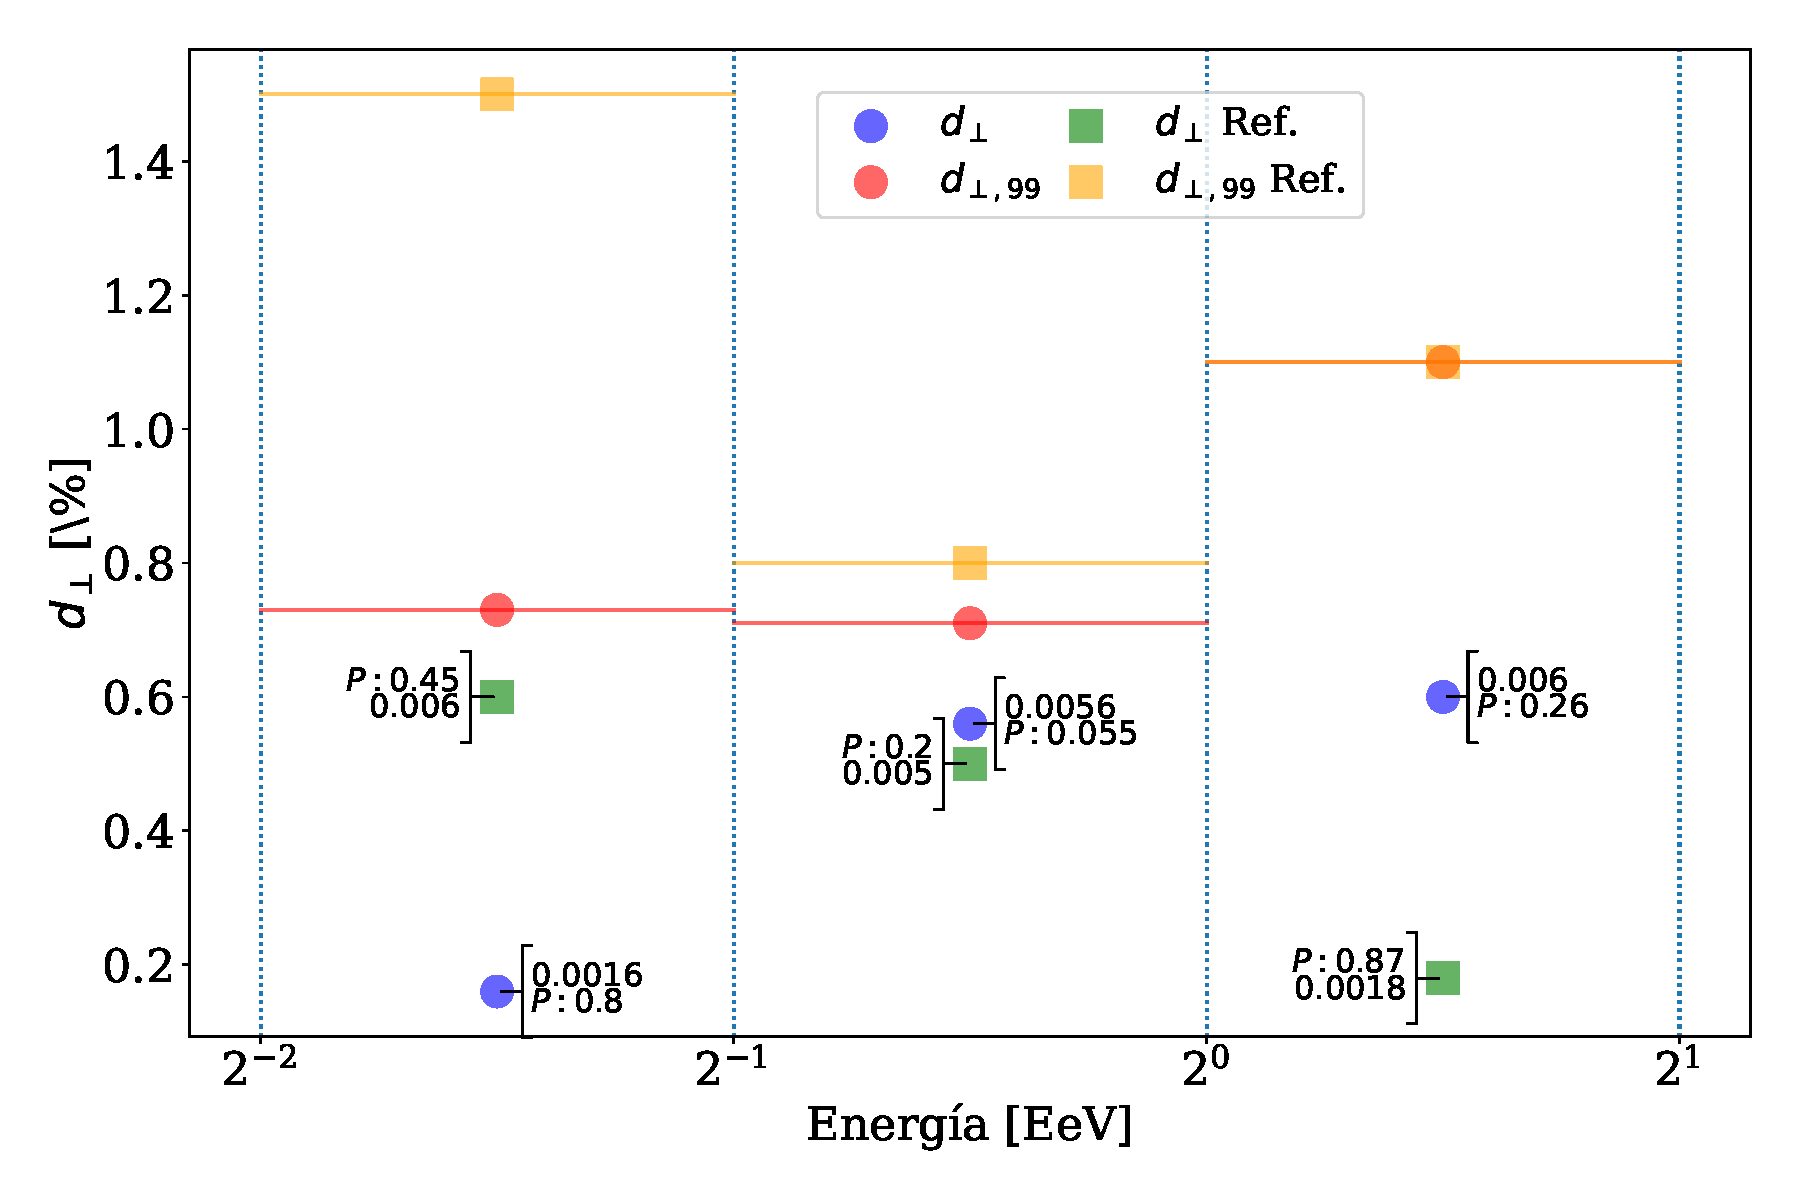
\includegraphics[width=0.75\textwidth]{Figs/d_perp_no_normalizado_v4.pdf}
    %         \end{center}
    %         \caption{Sin normalizar}
    %         \label{fig:no_normalizado}
    %     \end{small}
    % \end{figure}
    
    % Para compararlos mejor con respecto a $d_{\perp,UL}$, usamos el valor de cada rango y de cada conjunto de datos, para normalizar la amplitude de $d_{\perp,UL}$. Como se muestra en la Fig.\ref{fig:normalizado}, ahora $d_{\perp,UL}=1$ y los otros valores se pueden comparar. 

    % \begin{figure}[H]
    %     \begin{small}
    %         \begin{center}
    %             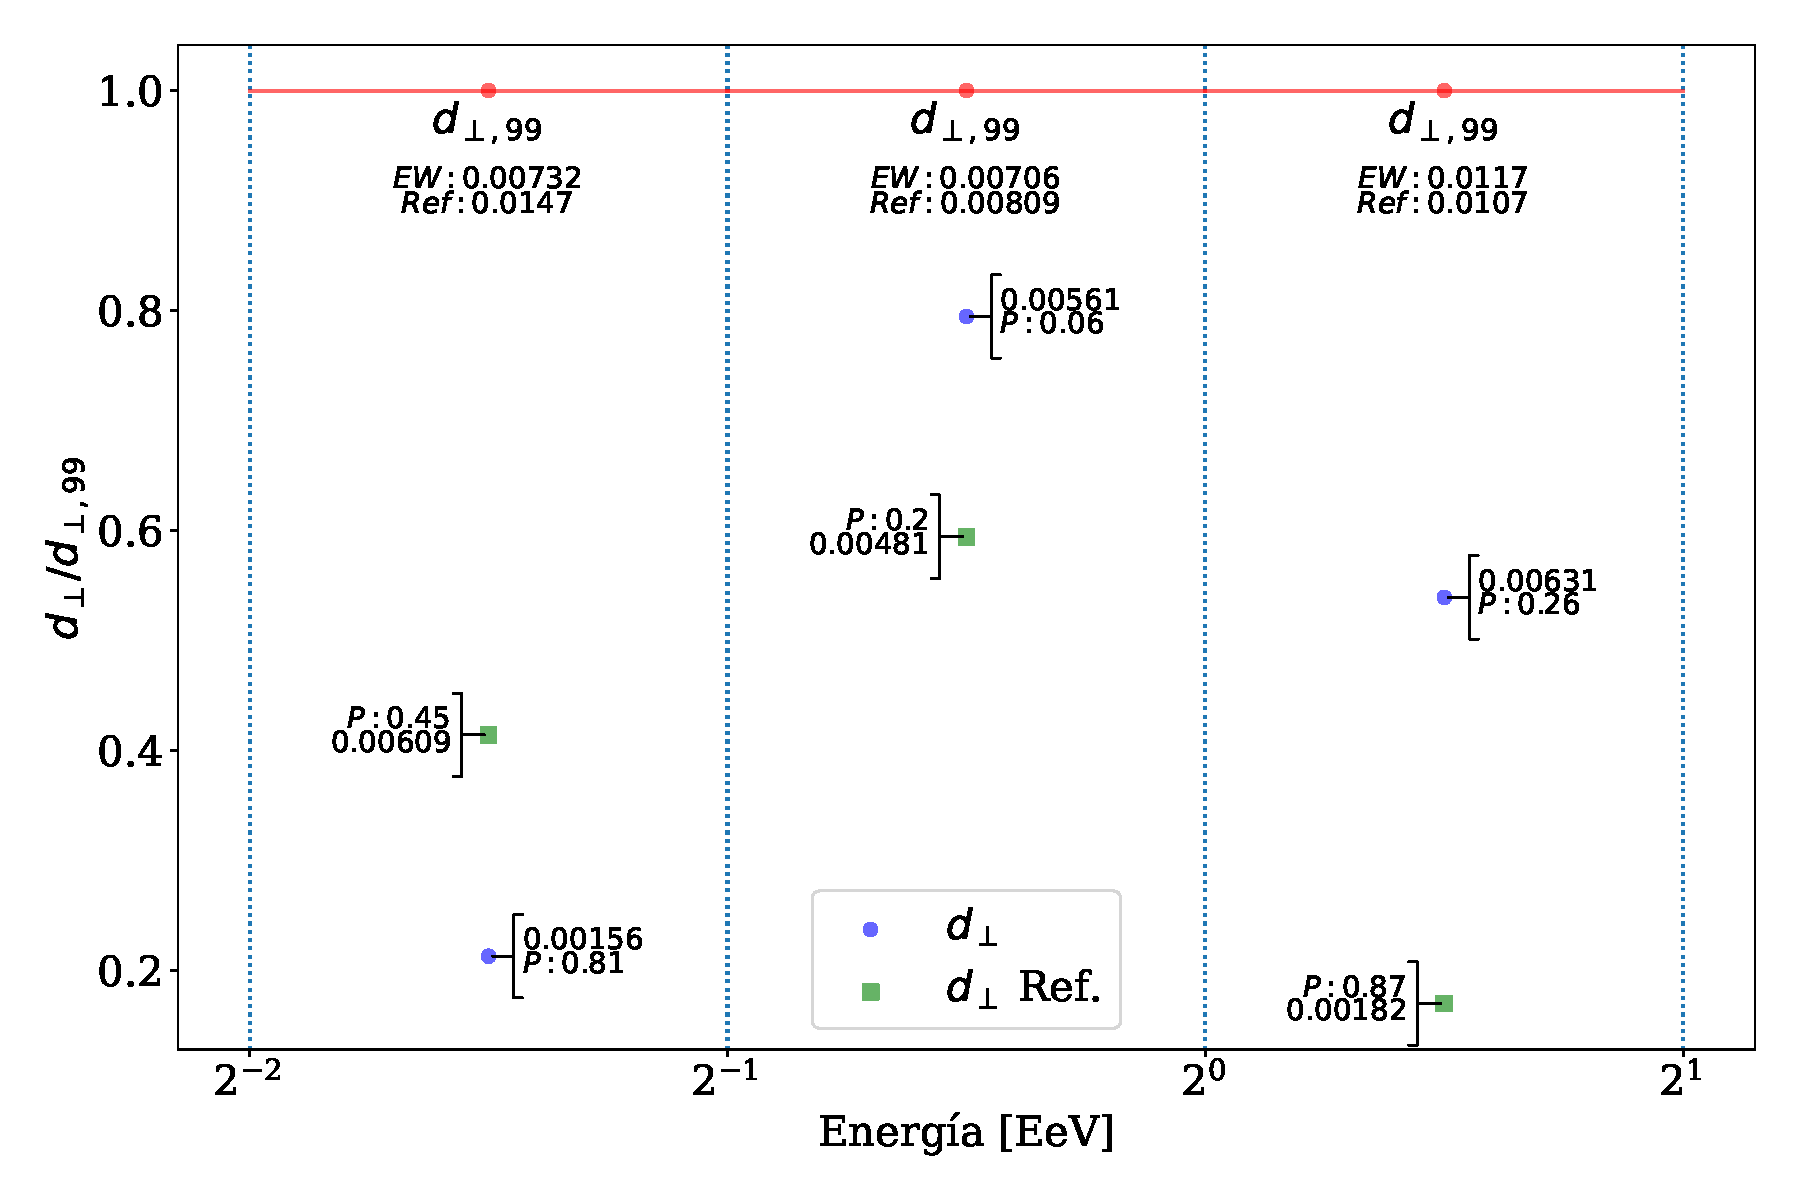
\includegraphics[width=0.75\textwidth]{Figs/d_perp_normalizado.pdf}
    %         \end{center}
    %         \caption{Valores normalizados con $d_{\perp,UL}$}
    %         \label{fig:normalizado}
    %     \end{small}
    % \end{figure}

    Una forma  para poder comparar los resultados de $d_\perp$ calculados de distintos conjuntos de  datos entre sí, es dividir estos valores con  sus respectivos $\sigma_{x,y}$. De esta manera, podemos comparar cuan apartados están con respecto $\sigma_{x,y}$. De esta manera se obtiene la Fig.\ref{fig:normalizado_sigma}, donde podemos decir que en los rangos entre 0.5 EeV - 1.0 EeV y 1.0 EeV - 2.0 EeV, la amplitude obtenida en este trabajo utilizando los eventos de All Triggers es más significativa que los resultados obtenidos por el trabajo \cite{Aab_2020} con el Disparo Estándar. Estos resultados difieren de trabajo \cite{Aab_2020} por $\sim 1\sigma_{x,y}$ y $\sim 2 \sigma_{x,y}$ respectivamente. Para comparar los resultados en el  rango 0.25 EeV - 0.5 EeV, tenemos que tener en cuenta que el Disparo Estándar tiene una sensibilidad menor que el All Triggers. Esto se ve claramente en la Tabla \ref{tab:datasets}, donde el primero tiene 7 veces menos eventos para analizar que el segundo. Por lo tanto, la discrepancia entre este trabajo y los resultados presentados en \cite{Aab_2020} puede deberse a la  diferencia de eventos a estudiar causada por la sensibilidad del disparo.

    \begin{figure}[H]
        \begin{small}
            \begin{center}
                \vspace*{-0.21 cm}
                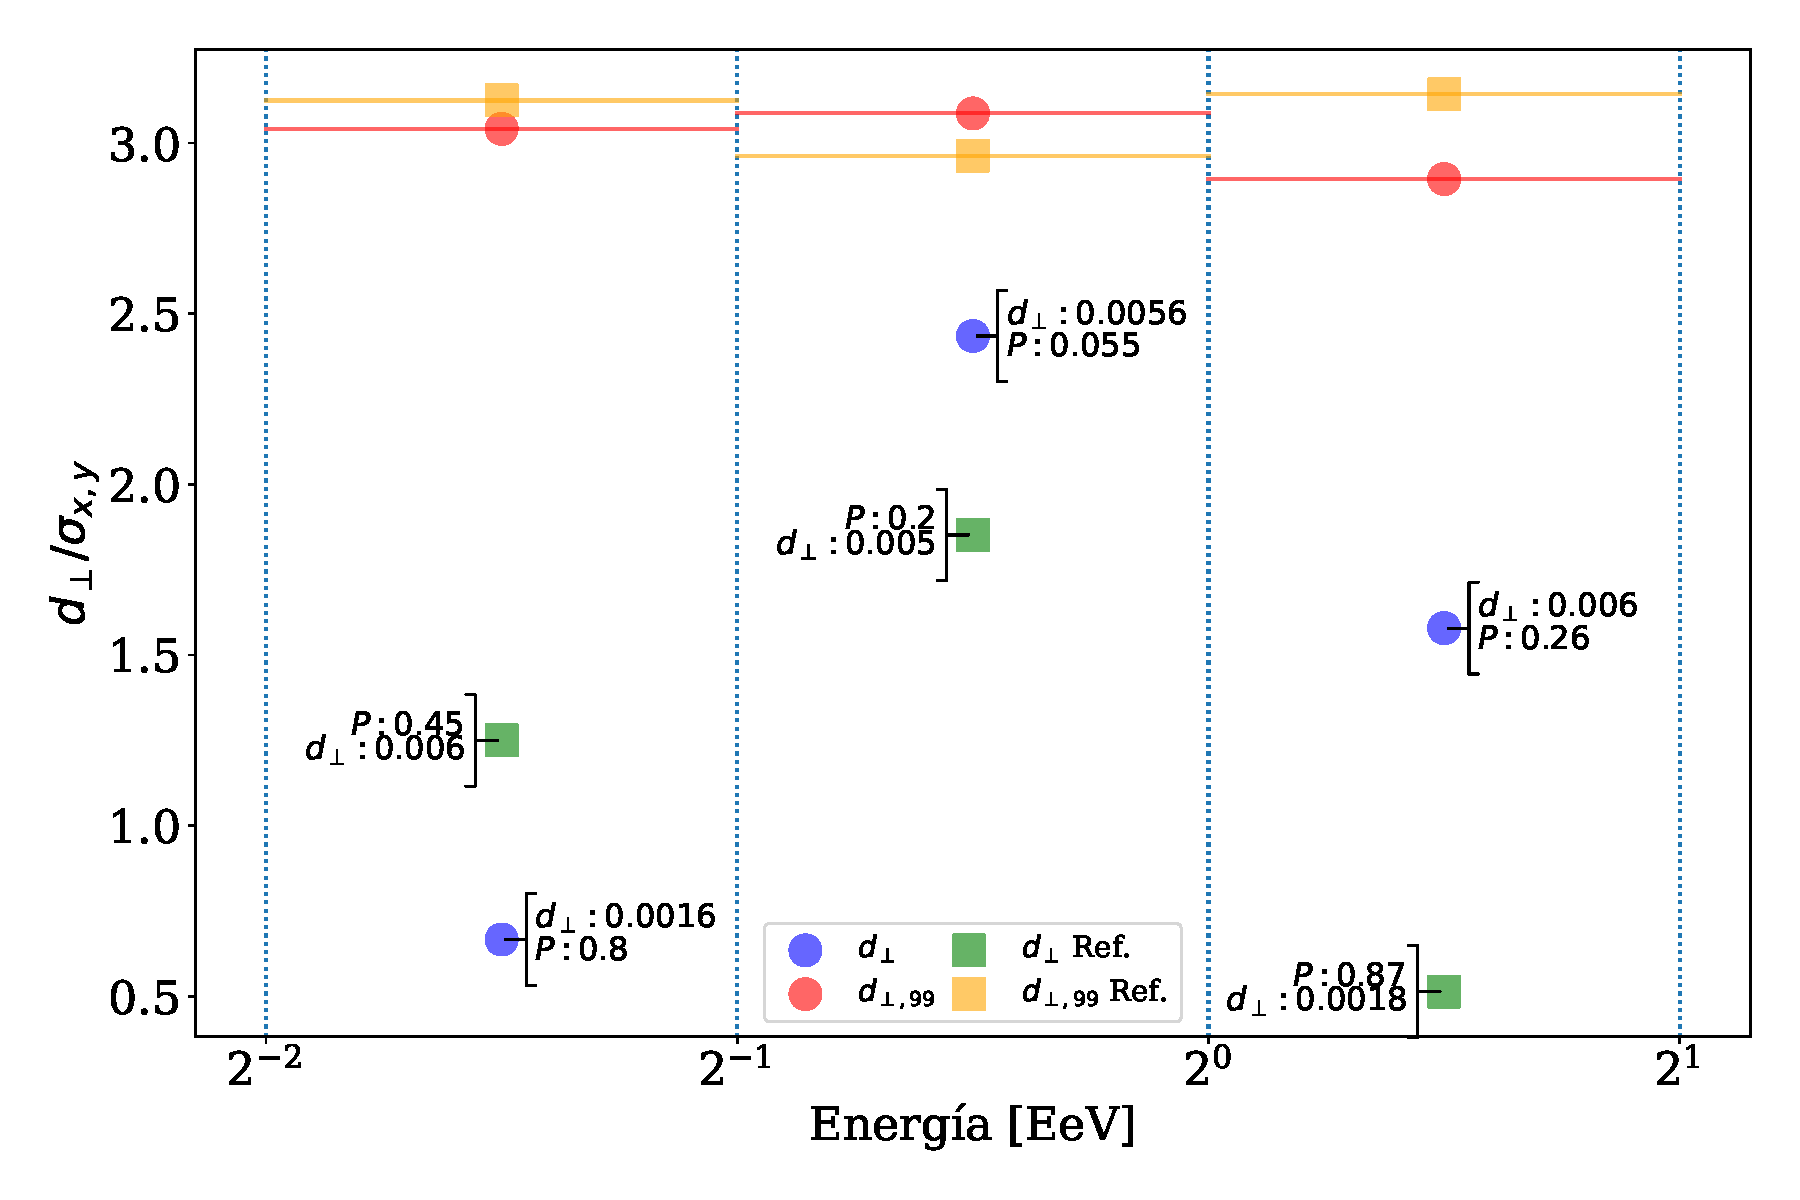
\includegraphics[width=\textwidth]{Figs/d_perp_normalizado_sigmas_v6.pdf}
                \vspace*{-1 cm}
            \end{center}
            \caption{Variaciones de la amplitude $d_\perp$ con respecto a $\sigma_{x,y}$ comparados con $d_{\perp,99}$ para distintos rangos de energía. Estos valores son obtenidos con el método East-West. }
            \label{fig:normalizado_sigma}
        \end{small}
    \end{figure}



    Considerando los valores de $\sigma_{x,y}$ y $d_\perp$ obtenidos para cada rango de energía y con los métodos Rayleigh y East-West, es posible  comparar las direcciones, valores e incertidumbres en la Fig.\ref{fig:incertidumbre}. Las líneas punteadas están centradas en los valores reportados  en cada rango de energía por el trabajo \cite{Aab_2020}, obtenido con el Disparo Estándar. El  radio de cada círculo punteado igual al $\sigma_{x,y}$ de cada rango de energía. Los círculos sombreados indican el rango de incertidumbre  a $1\sigma_{x,y}$ de los valores obtenidos en este trabajo utilizando All Triggers. Cada flecha dentro de estos círculos sombreados indica a dirección y valor de $d_\perp$.    El punto asociado al método Rayleigh corregido con la modulación del clima de All Triggers en el rango 1-2 EeV se denota con \emph{Ray,mod}.


    En los rangos de energía 0.25 EeV - 0.5 EeV y 0.5 EeV - 1.0 EeV, los valores obtenidos con All Triggers y el Disparo Estándar son compatibles entre sí dentro de la incertidumbre, además de contener la dirección al centro galáctico dentro de sus incertidumbres. Esto es interesante de resaltar ya que es esos rangos de energía, se espera que los rayos cósmicos sean galácticos.

    En el rango 1.0 EeV - 2.0 EeV, se comparan resultados para el método de Rayleigh (\emph{Ray}) y el método East-West (\emph{EW}) obtenidos con All Triggers, y el valor obtenido por la Colaboración en el trabajo \cite{Aab_2020} mediante el método Rayleigh con el Disparo Estándar. Todos estos resultados son compatibles entre sí dentro de $1\sigma_{x,y}$ de incertidumbre. 

\begin{figure}[H]
    \begin{small}
        \begin{center}
            \vspace*{-0.21 cm}
            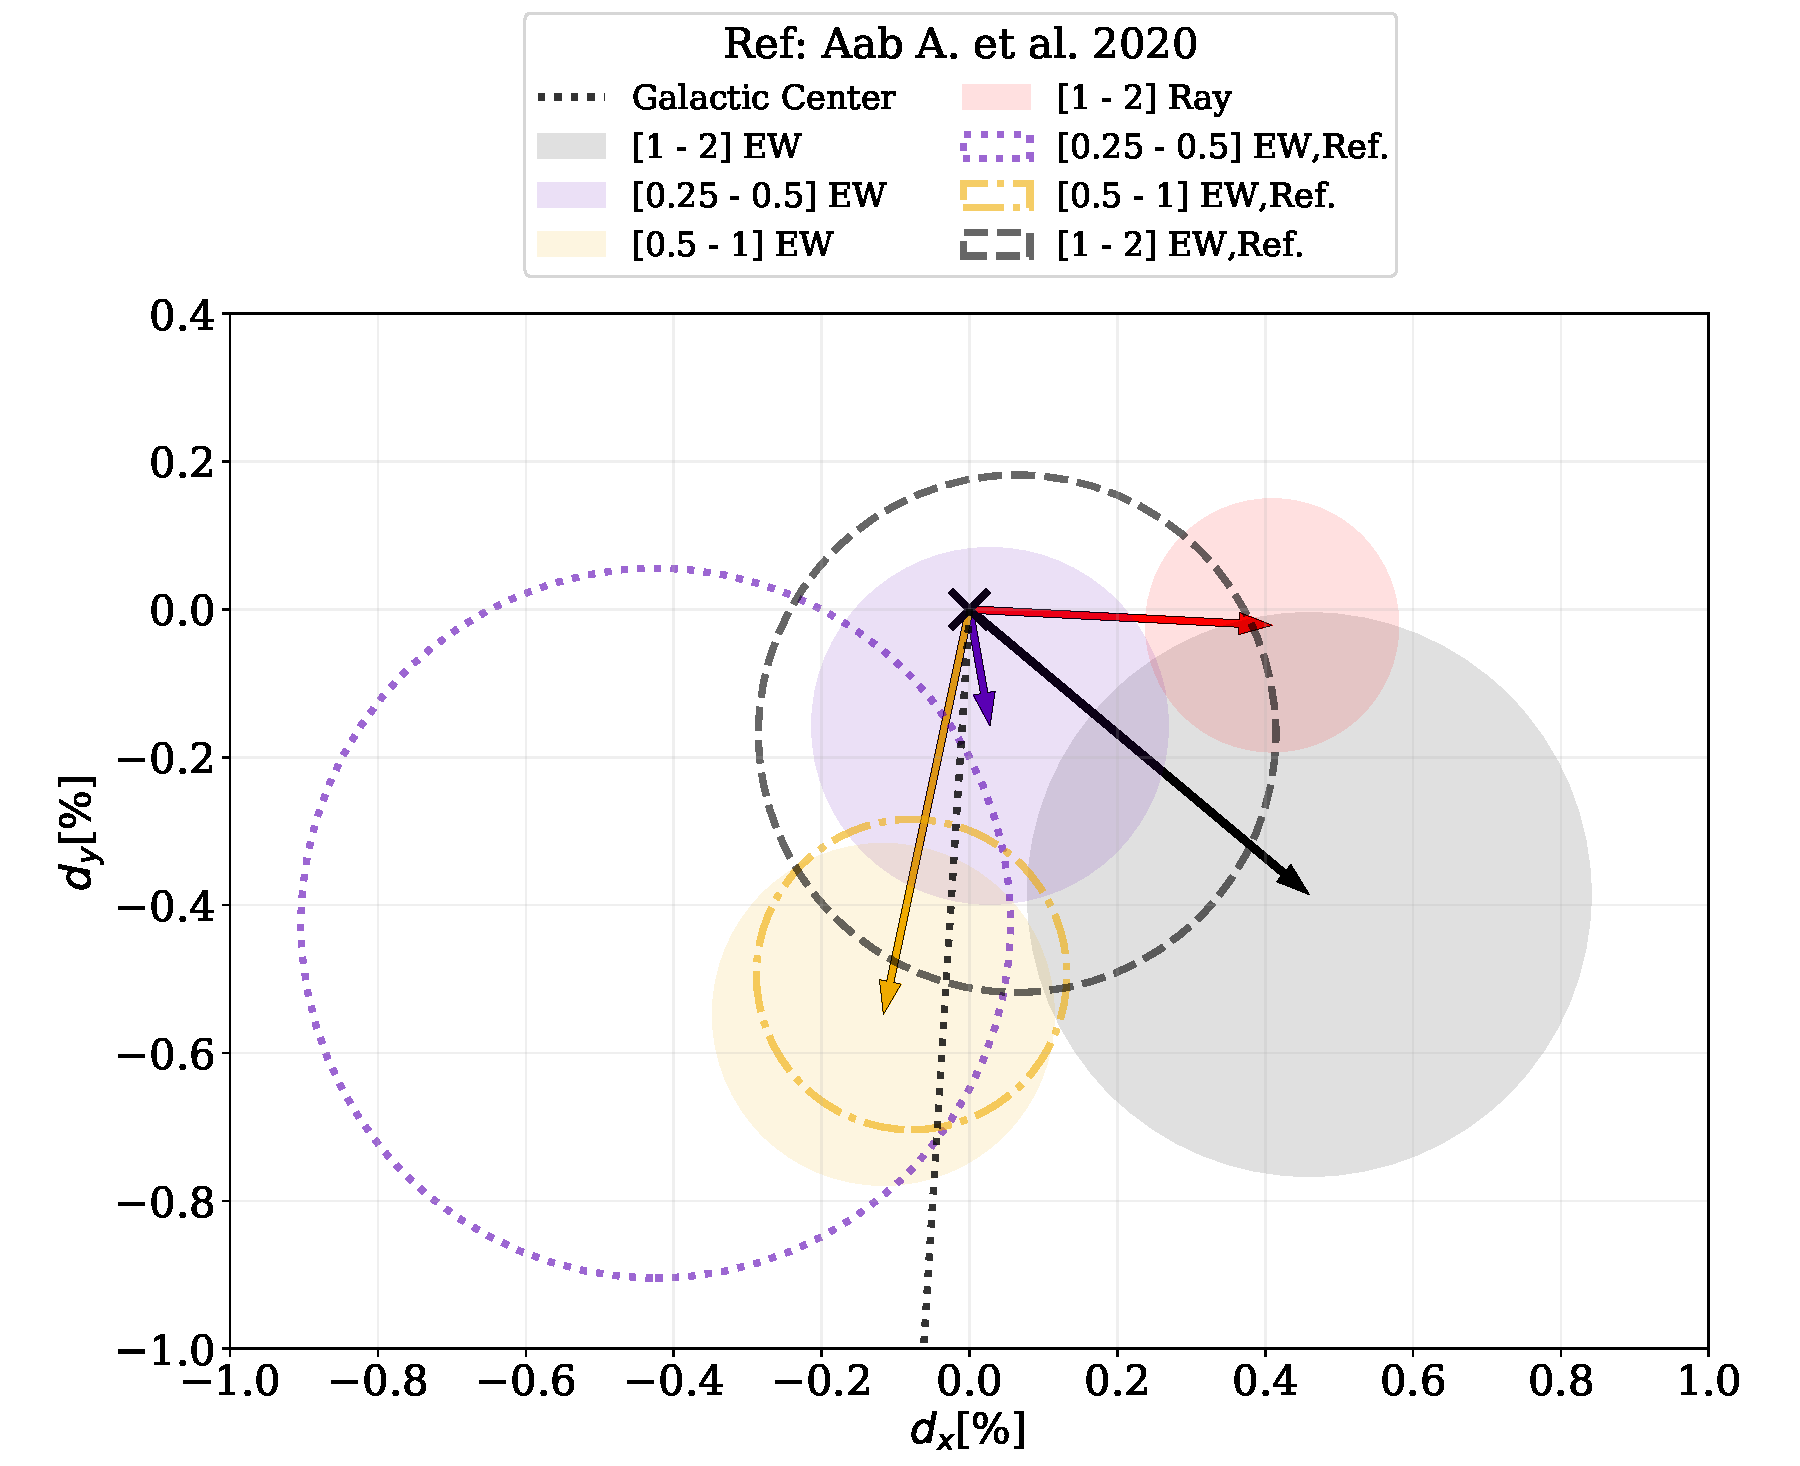
\includegraphics[width=\textwidth]{Figs/comparando_sigmas_v4.pdf}
            \vspace*{-1. cm}
        \end{center}
        \caption{Amplitudes con incertidumbre, apuntando en la dirección  de la phase. Los círculos punteados los valores del trabajo Aab A. et al. (2020) \cite{Aab_2020} con sus respectivas incertidumbres y la línea punteada en negro marca la dirección del centro galáctico.}
        \label{fig:incertidumbre}
    \end{small}
\end{figure}



\begin{thebibliography}{9}
    
  \bibitem{resolucion_barrido}
  Abreu, P., Aglietta, M., Ahn, E., Albuquerque, I., Allard, D., Allekotte, I.,
    \emph{et~al.}
   Search for first harmonic modulation in the right ascension
    distribution of cosmic rays detected at the pierre auger observatory.
   \emph{Astroparticle Physics}, \textbf{34}~(8), 627 -- 639, 2011.
   \bibitem{taborda}
    Taborda, O. {Estudios de anisotropías a grandes escalas angulares de los rayos
  cósmicos de alta energía detectados por el observatorio Pierre Auger}. PhD thesis, Instituto Balseiro, 2018. 
   
   \bibitem{Aab_2020}
    {Aab A. et al.},{Cosmic-Ray Anisotropies in Right Ascension Measured by the {Pierre   Auger Observatory}}.
    \emph{The Astrophysical Journal}, \textbf{891}~(2), 142, 2020. \url{https://doi.org/10.3847/1538-4357/ab7236}.
    \bibitem{codigo}  
    {Code used in \cite{Aab_2020}}.
\end{thebibliography}
    

\end{document}